\documentclass[a4paper,12pt,twoside]{scrreprt}
% Autor der Vorlage: Klaus Rheinberger, FH Vorarlberg, 2017-02-20

% Pakete:
\usepackage[utf8]{inputenc}
\usepackage[T1]{fontenc} % Silbentrennung bei Sonderzeichen
\usepackage{graphicx} % Bilder einbinden
\usepackage{wrapfig} % Bilder positionieren
\usepackage[ngerman]{babel} % Deutsche Sprachanpassungen
\usepackage{minted} % Code Highlighting/Import
\usepackage{csquotes} % Anführungszeichen und Zitieren
\usepackage{acronym} % Abkürzungsverzeichnis
\usepackage[bindingoffset=8mm]{geometry} % Bindeverlust von 8mm einbeziehen
\usepackage{caption} % Abbildungslegenden
\usepackage{xcolor} % Farbige Hervorhebungen
\usepackage{setspace} % Zeilenabstand
\usepackage[style=authoryear,citestyle=authoryear,backend=biber]{biblatex} % Literaturverweise
\usepackage[
    linktocpage=true,
    pdfauthor={Dominic Luidold},
]{hyperref} % Links -> \href{https://www.wikibooks.org}{Wikibooks home}

% Einstellungen:
\captionsetup{format=hang, justification=raggedright}
\addbibresource{Zotero.bib}
\setcounter{secnumdepth}{4}
\setcounter{tocdepth}{4} % Tiefe der Gliederung im Inhaltsverzeichnis

% Custom Commands
\renewcommand{\listingscaption}{Quellcode}
\renewcommand\listoflistingscaption{Quellcodeverzeichnis}

% Dokumentenbeginn
\begin{document}
\onehalfspacing % Zeilenabstand 1,5

% Sperrvermerkseite
\thispagestyle{empty}

\section*{Sperrvermerk}
\label{sec:sperrvermerk}
Auf Wunsch der Firma Fusonic GmbH, im Auftrag der Viterma Handels GmbH, ist die vorliegende Arbeit bis zum [DATUM] für die öffentliche Nutzung zu sperren.

Veröffentlichung, Vervielfältigung und Einsichtnahme sind ohne ausdrückliche Genehmigung der oben genannten Firma und dem Verfasser nicht gestattet. Der Titel der Arbeit sowie das Kurzreferat/Abstract dürfen jedoch veröffentlicht werden.

\vspace{3cm}

\noindent Dornbirn, am [Datum] \hfill Unterschrift des Verfassers (Dominic Luidold)

\vspace{2cm}

\hfill Firmenstempel\hspace{2cm}

% Titelblatt:
% \newpage\mbox{}\newpage
\cleardoublepage % force output to a right page
\thispagestyle{empty}
\begin{titlepage}
    \begin{flushright}
    
\includegraphics[width=0.4\linewidth]{images/Logo_FHV.jpg}
    \end{flushright}
    \begin{flushleft}
    \section*{[Titel der Arbeit]}
    \subsection*{[Untertitel der Arbeit]}
    \vspace{1cm}

    Bachelorarbeit I\\
    zur Erlangung des akademischen Grades
    \vspace{0.5cm}

    \textbf{Bachelor of Science in Engineering (BSc)}

    \vspace{1cm}
    Fachhochschule Vorarlberg\newline
    Informatik – Software and Information Engineering

    \vspace{0.5cm}

    Betreut von\newline
    Prof. (FH) Dipl. Inform. Thomas Feilhauer

    \vspace{0.5cm}

    Vorgelegt von\newline
    Dominic Luidold\newline
    Dornbirn, [Datum]
    \end{flushleft}
\end{titlepage}

% Widmung:
\newpage
\section*{Widmung}
\label{sec:widmung}
Trotz des Sperrvermerks, an der diese Arbeit gebunden ist, möchte ich es mir nicht nehmen lassen, den Personen einen Dank auszusprechen, die mich bei der Umsetzung und Realisierung meiner Bachelorarbeit I unterstützt haben.

\medskip

Zu Beginn möchte ich meinen Betreuern Thomas Feilhauer (Fachhochschule Vorarlberg) und Michael Zangerle (Fusonic GmbH) danken, die jederzeit ein offenes Ohr für Fragen, Anliegen und Unklarheiten hatten. Durch ihre fachliche Kompetenz, ihre langjährige Erfahrung sowie ihr Know-how konnte ich vieles lernen, das ich in mein weiteres Berufsleben mitnehmen kann.

\medskip

Als nächstes möchte ich meiner gesamten Familie danken, denen ich während des Schreibens dieser Arbeit wahrscheinlich mehr als nur einmal auf die Nerven gegangen bin. Nur durch die Tatkräftige Unterstützung mit Snacks, Süßigkeiten und dem besten Zimmerservice der Welt konnte ich so ungestört an der Bachelorarbeit schreiben. Ohne ihr Korrekturlesen wären zudem mehr Tippfehler vorhanden als mir lieb sind und ich auf meine Tastatur schieben kann.

\medskip

Zu guter Letzt möchte ich meine Arbeit all jenen widmen, die für die Gleichbehandlung und Gleichberechtigung aller kämpfen, sich für eine Sache einsetzen, die größer als sie selbst ist und für die sie teilweise sogar ihr Leben aufs Spiel setzen. Auch 2020 braucht es weltweit immer noch laute Stimmen - Stimmen, die sich nicht unterkriegen lassen.

\bigskip

\begin{quote}
    \begin{flushright}
        \textit{\enquote{The time is always right to do what is right.}}\\
        Dr. Martin Luther King Jr.
    \end{flushright}
\end{quote}

% Kurzreferat:
\newpage
\section*{Kurzreferat}
\label{sec:kurzreferat}

\subsection*{[Deutscher Titel Ihrer Arbeit]}

[Text des Kurzreferats]

% Abstract:
\newpage
\section*{Abstract}
\label{sec:abstract}

\subsection*{[English Title of your thesis]}

[text of the abstract]

% Vorwort:
\newpage
\section*{Vorwort}
\label{sec:vorwort}

Der Verfasser der vorliegenden Arbeit bekennt sich zu einer geschlechtergerechten Sprachverwendung.

Um die Lesbarkeit zu gewährleisten und zugunsten der Textökonomie werden die verwendeten Personen beziehungsweise Personengruppen fix männlich oder weiblich zugeordnet. Zum Beispiel wird immer \enquote{die Entwicklerin} und \enquote{der Benutzer} verwendet. Es wurde besonders darauf geachtet, stereotype Rollenbeschreibungen zu vermeiden. Die insgesamt eventuell dadurch hervorgerufene Irritation bei den Lesenden ist gewünscht und soll dazu beitragen, eine Bewusstheit für die bestehende, Frauen diskriminierende Sprachgewohnheit (generelle Verwendung der männlichen Begriffe für beide Geschlechter) zu wecken beziehungsweise zu stärken.

% Inhaltsverzeichnis:
\cleardoublepage % force output to a right page
\tableofcontents

\clearpage
\phantomsection
\addcontentsline{toc}{chapter}{Abbildungsverzeichnis}
\listoffigures

% Abkürzungsverzeichnis:
\clearpage
\phantomsection
\addcontentsline{toc}{chapter}{Abkürzungsverzeichnis}
\chapter*{Abkürzungsverzeichnis}
\begin{acronym}
 \acro{API}{Application Programming Interface}
 \acro{BLS}{Better Life System}
 \acro{CI}{Continuous Integration}
 \acro{CD}{Continuous Deployment}
 \acro{CQS}{Command Query Separation}
 \acro{CQRS}{Command Query Responsibility Segregation}
 \acro{CRUD}{Create, Read, Update, Delete}
 \acro{DTO}{Data Transfer Object}
 \acro{IDE}{Integrierte Entwicklungsumgebung}
 \acro{JSON}{JavaScript Object Notation}
 \acro{LTS}{Long Term Support}
 \acro{MVC}{Model View Controller}
\end{acronym}

\chapter{Einleitung}
\label{chap:einleitung}
Diese Bachelorarbeit verfolgt das Ziel, einen Einblick in die Implementierung und Erweiterung des bereits bestehenden Backend-Systems des \enquote{Better Life System} (kurz \enquote{BLS}) der Viterma Handels GmbH mit dem sogenannten \enquote{CQRS}-Pattern zu geben.

Das Better Life System - welches von Fusonic GmbH entwickelt wird und mittels einer Weboberfläche und gängigen Webbrowsern bedient werden kann - ermöglicht es Endkunden, mithilfe einer Handelsvertreterin der Firma Viterma (beziehungsweise mit einer Vertreterin eines ihrer Franchise-Partner) ein Badezimmer anhand der jeweiligen Bedürfnisse auszusuchen und zu konfigurieren, um sich schlussendlich ein entsprechendes Angebot dafür erstellen zu lassen.

\section{Arbeitgeber Fusonic GmbH}
\label{sec:arbeitgeber}
Die Fusonic GmbH hat ihren Firmensitz in Götzis, Vorarlberg, und besteht aus einem Team von aktuell mehr als 25 Angestellten, Softwareentwicklerinnen und Projektleiterinnen. Diese sind aufgeteilt in diverse kleinere Teams, die intern unter anderem \enquote{Duck-Team} beziehungsweise \enquote{Parrot-Team} genannt werden. Die Teams arbeiten dabei an jeweils eigenständigen Projekten und setzen diverse Technologien ein. Zu den verwendeten Technologien gehören unter anderem C\# mit .NET, PHP mit Symfony und JavaScript/TypeScript mit Angular \parencite[]["Übersicht aller Technologien"]{fusonic_gmbh_web_2020}. Während es regelmäßigen Austausch unter den Teams gibt, besteht jedes aus Frontend- sowie Backend-Entwicklern, da die meisten Projekte - aufgrund der zugrundeliegenden Anwendungsfälle - aus einem Web-Frontend sowie serverseitigen Backend bestehen.

\section{Nutzung \& Umfeld des \enquote{Better Life System}}
\label{sec:nutzung-umfeld}
Die Hauptaufgabe des Better Life System liegt darin, als computergestütztes und plattformunabhängiges Tool, Vertreterinnen rund um die Viterma Handels GmbH bei der Konfiguration und Zusammenstellung eines Badezimmers - zusammen mit dem Endkunden (meist Haus- beziehungsweise Wohnungsbesitzer oder Hotels) - zu unterstützen und diesen Vorgang zu erleichtern. Das BLS wird des Weiteren dazu verwendet, aktuelle und abgeschlossene Angebote zu verwalten, Produkte, Produktinformationen und dazugehörige Preisaufschläge zu pflegen und Kundendaten abzulegen. Zudem dient es als Kontrollinstanz für in Auftrag gegebene Sanierungen, um sicherzustellen, dass alle benötigten Materialen und Teile in entsprechenden Mengen vorhanden und kompatibel sind.

Die Nutzung des BLS findet zu großen Teilen auf mobilen Rechnern beziehungsweise Laptops statt, die während der Beratung und Betreuung von Kunden zum Einsatz kommen. Da nicht immer gewährleistet werden kann, dass eine aufrechte Internetverbindung besteht, ist die Offline-Fähigkeit bei gleichbleibender Nutzung im Webbrowser ein wichtiger Bestandteil des Web-Frontends.

Aufgrund der Anforderungen der Viterma Handels GmbH, dass das Better Life System offline ebenso wie online verwendet werden kann, basiert das Frontend auf dem TypeScript Web-Framework Angular\footnote{\href{https://angular.io/}{Angular (https://angular.io)}}, welches solch eine Funktionalität ohne eine Installation oder zusätzliche Voraussetzungen am Endgerät unterstützt. Im Gegensatz zu weniger komplex gehaltenen Frontends - die primär Daten darstellen, die vom Backend eingehen - ist dieses beim BLS für einen Großteil der Ablauflogik, Berechnung von Preisen und Generierung von diversen PDFs zuständig. Das Frontend wird, da der Fokus dieser Arbeit auf der Entwicklung im Backend der Anwendung liegt, in weiterer Folge jedoch nicht genauer beleuchtet und als gegeben angenommen. Es kann davon ausgegangen werden, dass eingehende Anfragen an das Backend aus Benutzereingaben beziehungsweise zeitlich gesteuerten Events resultieren.

\pagebreak

Das Backend, welches alle API-Anfragen bearbeitet und als Schnittstelle zur Datenbank dient, ist in der Programmiersprache PHP geschrieben und verwendet das Framework Symfony\footnote{\href{https://symfony.com/}{Symfony (https://symfony.com)}} sowie diverse \enquote{Bundles}, die darauf aufbauen. Ein detaillierterer Überblick über den Aufbau, bisher angewandte Konzepte sowie technische Begebenheiten werden in Kapitel~\ref{chap:stand-technik} ab Seite \pageref{chap:stand-technik} behandelt.

\medskip

Während die Nutzung des Better Life System auf allen Plattformen - die einen modernen Webbrowser anbieten - möglich ist, findet die Entwicklung primär auf der Linux-Distribution Ubuntu statt. Der Grund für diese Betriebssystemwahl ist damit zu erklären, dass sowohl die lokale Entwicklung als auch die Continuous Integration Umgebung (genutzt für automatisierte Tests) und das Continuous Deployment mittels Docker\footnote{\href{https://docker.com}{Docker (https://docker.com)}} Containern stattfindet. Für die Entwicklung im Backend-Bereich der Anwendung wird die IDE PhpStorm verwendet, während im Frontend auf Visual Studio Code gesetzt wird.

\section{Problemstellung}
\label{sec:problemstellung}
Die Entwicklung des BLS hat im Frühjahr 2017 begonnen und die Anwendung ist seit dem stetig weiterentwickelt worden. Über die Zeit haben sich entsprechend sowohl die Anforderungen und Wünsche des Kunden als auch die technischen Begebenheiten, Best Practices und Möglichkeiten verändert.

Die bisher bei der Umsetzung des Projekts verwendete Struktur sowie der Aufbau wurde stark an die empfohlene Herangehensweise von Symfony angelehnt und die Code-Basis entsprechend darauf ausgelegt \parencite[siehe dazu][\enquote{Use the Default Directory Structure}]{symfony_symfony_2020}. Durch wachsende Anforderungen und entsprechend benötigten Programmcode, der diese erfüllt, hat sich jedoch ein komplexes System ergeben, dessen \textit{Controller}, \textit{Entities}, \textit{Manager (Services)} und \textit{Data Transfer Objects (DTOs)} auf viele Verzeichnisse und Unterverzeichnisse verteilt sind. Die Abbildung~\ref{fig:ordnerstruktur} auf Seite \pageref{fig:ordnerstruktur} zeigt einen Ausschnitt von Ordnern die im Projekt vorkommen und jeweils alle Klassen ihrer Art beinhalten (im Verzeichnis \enquote{Controller} befinden sich, um ein Beispiel zu nennen, alle Controller des Projekts).

\begin{figure}[ht]
    \centering
    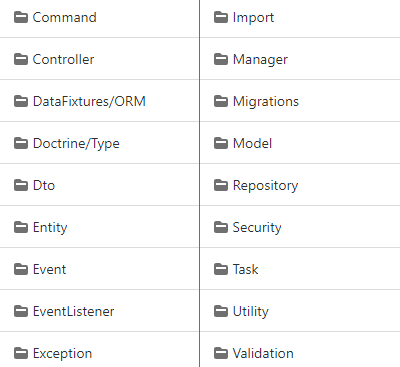
\includegraphics[scale=0.75]{images/bls_folder_structure.png}
    \caption{Teilausschnitt der BLS-Ordnerstruktur}
    \label{fig:ordnerstruktur}
\end{figure}

Durch die bisher gewählte Herangehensweise und den entsprechenden Aufbau hat sich jedoch ergeben, dass eine logische Gruppierung beziehungsweise Kapselung von zusammengehörenden Klassen, Controllern, Managern etc. eines API Endpunkts nur schwer möglich ist. Das hat zur Folge, dass das System an manchen Stellen sehr komplex aufgebaut ist und externe Personen eine gewisse Zeit brauchen, um sich mit internen Abläufen vertraut machen zu können. Neben der Verständlichkeit ist dadurch in weiterer Folge auch die Wartbarkeit und einfache Erweiterbarkeit im Falle von neuen Funktionalitäten nicht im vollen Ausmaß gegeben. Auf das Testen einzelner Bestandteile mittels sogenannter \textit{Unit Tests} wird im gesamten Projekt gesetzt. Primär werden beim Better Life System \textit{Smoke Tests} sowie \textit{Funktionale Tests} verwendet, die im Problemfall darauf hindeuten können, wo ein Fehler aufgetreten ist.

Da sich die Anforderungen an das Backend auch in Zukunft noch weiterentwickeln können und eine Skalierung der Infrastruktur beziehungsweise Abspaltung einzelner Teile (in sogenannte Microservices) nicht ausgeschlossen werden kann, bedarf es Möglichkeiten, dies möglichst effektiv und ohne großen, zusätzlichen Aufwand umsetzen zu können. Die von Symfony empfohlene Herangehensweise kann dies dabei nur bedingt unterstützen, was auch in diesem Fall einen limitierenden Faktor darstellt.

\section{Anforderungen}
\label{sec:anforderungen}
Die in Abschnitt~\ref{sec:problemstellung} angeführten Umstände und den daraus resultierenden Herangehensweisen, die nicht mehr in vollem Maße zufriedenstellend sind, führen zu neuen Anforderungen an das Better Life System. Diese sollen entsprechend umgesetzt werden, um ein zukunftssicheres Backend für die gesamte Anwendung garantieren zu können und die Entwicklung neuer sowie bestehender Funktionalitäten zu erleichtern und zu vereinheitlichen.

\medskip

Zum Start des Berufspraktikums Anfang Juli 2020 stand bereits fest, dass in weiterer Folge das CQRS-Pattern (was für \textit{Command Query Responsibility Segregation} steht) zum Einsatz kommen wird. Andere Projekte der Fusonic GmbH, die primär auf C\# und .NET basieren, haben bereits gute Erfahrungen damit gemacht und gehen deshalb davon aus, dass der Einsatz des Patterns die Qualität der bestehenden Code-Basis verbessern wird.

\medskip

Die Anforderungen, die im Zuge des Berufspraktikums und folglich dieser Bachelorarbeit zu erfüllen sind, bestehen darin, das aktuell bestehende System, neben dem \enquote{Tagesgeschäft} (sprich Bugfixes, Feature Requests etc.), laufend umzustellen und neue Funktionalitäten entsprechend mit der neuen Struktur und dem Pattern umzusetzen.

\section{Zielsetzung}
\label{sec:zielsetzung}
Die in den Abschnitten~\ref{sec:problemstellung} und \ref{sec:anforderungen} angeführten Punkte ergeben folgende Ziele, die im Verlauf des Berufspraktikums - so weit wie möglich - umzusetzen sind.

\smallskip

\noindent
Als Ziele einzustufen sind:
\begin{itemize}
    \item Vorbereitung der bestehenden Infrastruktur auf CQRS in Zusammenarbeit mit Mitarbeitern der Fusonic GmbH
    \item Umstellung der bestehenden API Endpunkte auf CQRS bei Beibehaltung von möglichst viel Programmlogik
    \item Umsetzung neuer Funktionalitäten mittels CQRS
    \item Abwickeln des Tagesgeschäfts
\end{itemize}

\chapter{Stand der Technik}
\label{chap:stand-technik}
Das folgende Kapitel gibt einen Überblick über den aktuellen Stand des Backends des Better Life System, dessen technischem Aufbau und dem zugrundeliegenden Konzept. Anschließend wird die von Symfony vorgeschlagene Architektur beleuchtet und auf das zukünftig eingesetzte CQRS-Pattern eingegangen. Am Ende des Kapitels werden die gängige Schichtenarchitektur und CQRS gegenübergestellt und Vor- sowie Nachteile aufgezeigt.

\section{Aufbau des Backends}
\label{sec:aufbau-backend}
Das Backend des BLS basiert auf der Programmiersprache PHP und setzt hierbei auf die zum aktuellen Zeitpunkt (Stand August 2020) neueste Version \textit{PHP 7.4}. Zur Verwaltung benötigter Abhängigkeiten kommt das Paketverwaltungssystem Composer\footnote{\href{https://getcomposer.org}{Composer (https://getcomposer.org)}} zum Einsatz, welches alle benötigten Symfony Bundles und anderweitige Packages - sowohl im Produktivsystem als auch während der Entwicklung - zur lokalen Installation sowie Nutzung zur Verfügung stellt.

Als Grundgerüst für das Backend dient das PHP-Framework Symfony in der LTS-Version \textit{4.4}, wobei zum Zeitpunkt des Verfassens dieser Arbeit Vorbereitungen für einen Umstieg auf Version \textit{5.x} getroffen werden. Das Backend dient als Schnittstelle zwischen dem Angular-Frontend und einem Datenspeicher, wobei hierfür eine relationale Datenbank auf Basis von MySQL eingesetzt wird. Um von Symfony aus auf die Datenbank zugreifen zu können, wird Doctrine\footnote{\href{https://www.doctrine-project.org}{Doctrine (https://www.doctrine-project.org)}} eingesetzt, welches ein objektrelationales Mapping vornimmt und in der Anwendung zur Verfügung stellt.

Der grundsätzliche Aufbau des Symfony Backends entspricht aktuell der empfohlenen Vorgehensweise laut Symfony Dokumentation und wird im nachfolgenden Abschnitt~\ref{sec:standard-schichtenarchitektur} erläutert.

\section{Gängige Schichtenarchitektur}
\label{sec:standard-schichtenarchitektur}

Symfony ist ein Webframework, welches aus vielen verschiedenen Komponenten und Bundles besteht, die alle unabhängig voneinander entwickelt werden. In Summe ergeben diese die Grundlage für eine Webapplikation auf Basis von PHP und werden auch von anderen Frameworks verwendet (beispielsweise Laravel\footnote{\href{https://laravel.com}{Laravel (https://laravel.com)}}, welches auf diversen Symfony-Komponenten basiert). Symfony orientiert sich dabei an der weit verbreiteten \textit{Model View Controller} Architektur (kurz \textit{MVC}) und bietet mittels flexiblem URI Routing, Session beziehungsweise Security Management und Logging unterstützende Funktionalitäten. \parencite[][]{tutorials_point_i_pvt_ltd_symfony_nodate-1}

\subsection{Empfohlener Ansatz}
\label{sub-sec:empfohlener-ansatz}
Symfony selbst gibt in der eigenen Dokumentation keine verpflichtenden Vorgaben an, wie genau man eine Applikation beziehungsweise Anwendung umsetzen soll. \parencite[][]{symfony_symfony_2020} Der Quellcode~\ref{code:symfony-project-structure} auf Seite \pageref{code:symfony-project-structure} zeigt den empfohlenen Aufbau einer Anwendung, bei der man die Anlehnung an das MVC-Pattern jedoch gut erkennen kann:

\begin{itemize}
    \item \textbf{Model:} Dem Model entsprechen die im \textit{Entity}-Verzeichnis abgelegten Klassen. Diese beinhalten das objektrelationale Mapping und können zusätzliche, domänenspezifische Funktionalitäten zur Verfügung stellen. Die Klassen, die im \textit{Repository}-Verzeichnis zu finden sind, stellen den Zugriff auf die Datenbank her und befüllen die Entities beziehungsweise Models mit Daten. \parencite[][]{tutorials_point_i_pvt_ltd_symfony_nodate}
    \item \textbf{View:} Im Falle der hier angenommenen Standardstruktur, wird der View-Teil mittels der Template Engine \textit{Twig} im gleichnamigen Verzeichnis abgehandelt. Im Falle des BLS ist dies mittels Data Transfer Objects gelöst, die bei den jeweiligen API Endpunkten als serialisierte JSON-Response zurückgegeben werden. \parencite[][]{tutorials_point_i_pvt_ltd_symfony_nodate}
    \item \textbf{Controller:} Die von der Namensgebung her am leichtesten zu erkennende Ähnlichkeit stellt das \textit{Controller}-Verzeichnis dar. Die darin vorhandenen Klassen werden verwendet, um eingehende Requests zu mappen. Diese Controller-Klassen sollten jedoch nur wenige Zeilen Code beinhalten, um Berechtigungen zu überprüfen sowie die Response zu erstellen. Die tatsächliche Businesslogik wird in separate Klassen aufgeteilt, die vom Controller aufgerufen werden, um diese möglichst zu entkoppeln. \parencite[][]{symfony_symfony_2020} Beim BLS liegt die Anwendungslogik beispielsweise in einem \textit{Manager}-Verzeichnis.
\end{itemize}

\begin{listing}[ht]
    \inputminted[fontsize=\footnotesize,linenos]{text}{code/symfony_directory_structure.txt}
    \caption[Von Symfony empfohlener Projektaufbau]{Von Symfony empfohlener Projektaufbau. Quelle: \cite[]{symfony_symfony_2020}}
    \label{code:symfony-project-structure}
\end{listing}

\subsection{Funktionsweise}
\label{sub-sec:standard-funktionsweise}
Die Funktionsweise der von Symfony vorgeschlagenen Architektur kann, unter Bezugnahme auf die in Abschnitt~\ref{sub-sec:empfohlener-ansatz} beschriebenen Prinzipien, mithilfe der Abbildung~\ref{fig:single-model-fowler} genauer beleuchtet werden.

\smallskip

Im Zuge der Entwicklung einer Webapplikation mit entsprechendem Backend oder einer API wird oftmals auf CRUD beziehungsweise einen CRUD-ähnlichen Aufbau gesetzt. Die Nutzung eines einzelnen Models, dem jeweiligen DTO (sofern vorhanden) sowie der dazugehörenden Businesslogik ist dabei ein einfacher Weg, um schnell und anfangs unkompliziert Funktionalitäten für die CRUD Anwendungsfälle umsetzen zu können. Auch bei weiterführenden Nutzungsfällen, bei denen beispielsweise mehrere Models zusammengeführt und entsprechend validiert werden müssen, wird die bestehende Logik herangezogen und keine spezifische Auftrennung von ausgeführten Aktionen vorgenommen. Dadurch entsteht jedoch eine Vermischung von lesenden und schreibenden Zugriffen in der Anwendungslogik sowie der Funktionalitäten der entsprechenden Models. \parencite[][]{fowler_cqrs_2011} Die Abbildung~\ref{fig:single-model-fowler} stellt diesen Umstand anschaulich im hellgrau hinterlegten Rechteck \enquote{Application} dar:

\begin{figure}[ht]
    \centering
    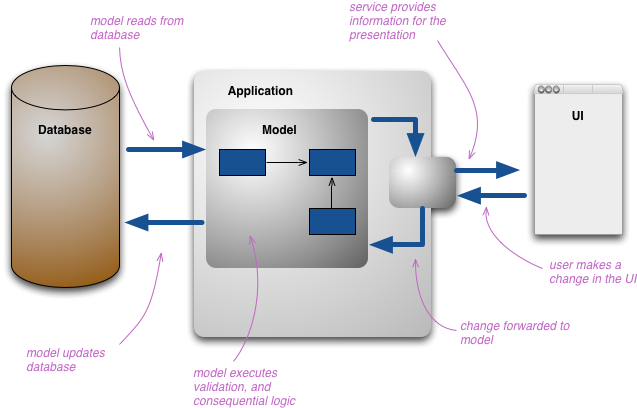
\includegraphics[scale=0.55]{images/fowler_single_model.png}
    \caption[Aufbau einer gängigen Schichtenarchitektur]{Aufbau einer gängigen Schichtenarchitektur.\\Quelle: \cite{fowler_cqrs_2011}}
    \label{fig:single-model-fowler}
\end{figure}

\section{CQRS Pattern}
\label{sec:cqrs-pattern}
Das Command Query Responsibility Segregation Pattern (nachfolgend CQRS genannt) soll als Grundlage für die zukünftige Struktur des Better Life System dienen. Die Entscheidung für den Wechsel auf dieses Pattern beziehungsweise die zugrundeliegende Architektur basiert primär auf Erfahrungswerten, die Fusonic GmbH bei anderen Projekten sammeln konnte. Der Einsatz dieses Patterns soll die im Kapitel~\ref{chap:einleitung} angesprochenen Problemstellungen in Angriff nehmen und die Komplexität, Verständlichkeit, Testbarkeit und Erweiterbarkeit des Systems langfristig verbessern.

Die bisherigen Erfahrungen, die Fusonic mit dieser Herangehensweise gemacht hat, basieren auf C\# und .NET Core Projekten. Ein entsprechender Einsatz mit der Programmiersprache PHP und dem Framework Symfony wurde bisher nur konzeptionell durchgeplant und findet damit erstmalig Einzug in ein Kundenprojekt.

\subsection{Grundlagen von CQRS}
\label{sub-sec:cqrs-grundlagen}
Um über das CQRS-Pattern sprechen zu können, werden einige grundlegende Begrifflichkeiten sowie Konzepte benötigt, die im weiteren Verlauf dessen Ursprung definieren und Verständnis schaffen sollen.

CQRS, beziehungsweise die Terme \textit{Command} und \textit{Query}, beziehen sich auf das Prinzip der \textit{Command Query Separation} (kurz \textit{CQS}). \parencite[][]{young_cqrs_2010} CQS definiert auf der einen Seite lesende und auf der anderen Seite schreibende Aktionen in einem System, die voneinander getrennt sind und unterschiedlich agieren sowie verschiedene Resultate als Folge haben:

\begin{itemize}
    \item Lesende Aktionen, sogenannte \textbf{Queries}, greifen auf Daten in einem System zu und liefern diese bei einem Aufruf als Ergebnis zurück. Durch das Ausführen der Aktion wird der Zustand eines Objekts oder des Systems im Ganzen nicht verändert. \parencite[][]{fowler_commandqueryseparation_2005}
    \item Schreibende Aktionen, sogenannte \textbf{Commands}, verändern Daten in einem System, führen jedoch zu keinem Rückgabewert. Durch das Ausführen der Aktion wird der Zustand eines Objekts oder des Systems im Ganzen bleibend verändert. \parencite[][]{fowler_commandqueryseparation_2005}
\end{itemize}

\noindent
Fowler beschreibt den Vorteil dieser Aufteilung damit, dass Methoden, die den Zustand eines Objekts oder Systems verändern, von denen logisch getrennt werden können, die nur lesend darauf zugreifen. Queries können dadurch \enquote{gefahrlos} und in beliebiger Reihenfolge an jeder Stelle in einer Anwendung eingesetzt werden, während dies bei Commands nicht gegeben ist. \parencite[][]{fowler_commandqueryseparation_2005}

\subsection{Funktionsweise von CQRS}
\label{sub-sec:cqrs-funktionsweise}
Die Funktionsweise des CQRS Konzepts basiert, wie im Abschnitt~\ref{sub-sec:cqrs-grundlagen} beschrieben, auf dem Einsatz von Commands und Queries. Durch deren Einsatz wird eine effektive Aufteilung in zwei separate und optimalerweise unabhängige Modelle erzielt, wodurch zum einen ein Fokus auf die jeweilige Verantwortlichkeit des Modells gelegt werden kann und zum anderen die übermäßige Optimierung hin zu einer Datenbank wegfällt. Dadurch rückt die Anwendungs- beziehungsweise Businesslogik deutlich mehr in den Vordergrund und kann entsprechend besser ausgebaut und getestet werden. \parencite[][]{heimeshoff_cqrs_2013}

\medskip

Anhand der Abbildung~\ref{fig:cqrs-fowler} auf Seite \pageref{fig:cqrs-fowler} wird verdeutlicht, wie der Ablauf in einem auf CQRS basierenden System abläuft:

\textbf{Ändern von Daten:} Eine vom Benutzer ausgelöste Änderung der Daten (im Falle des BLS durch eine Aktion im Angular-Frontend) führt dazu, dass diese an ein Command Model weitergeleitet werden. Das Model beinhaltet die Daten, die abgeändert und persistiert werden sollen und stellt diese gegebenenfalls einem Domänenmodell mit entsprechenden Funktionalitäten - auf Basis des Domain-Driven Designs - zur Verfügung \parencite[][]{heimeshoff_cqrs_2013}. Das Command Model, dass die Integrität der eingehenden Daten sichergestellt hat, wird abschließend in der Datenbank persistiert, womit die Aktion somit - im Regelfall ohne Rückgabewert - abgeschlossen wird. \parencite[][]{fowler_cqrs_2011}

\textbf{Abfragen von Daten:} Ein Abfragen der Daten (ebenfalls durch das Frontend ausgelöst) führt dazu, dass diese von der Datenbank geladen und mittels des Query Models (in manchen Fällen auch mehrerer) im entsprechenden Format serialisiert werden. Die Aktion wird damit abgeschlossen, dass die Daten nach außen als Rückgabewert(e) zurückgegeben oder dargestellt werden. \parencite[][]{fowler_cqrs_2011}

\vspace{0.5cm}

\begin{figure}[ht]
    \centering
    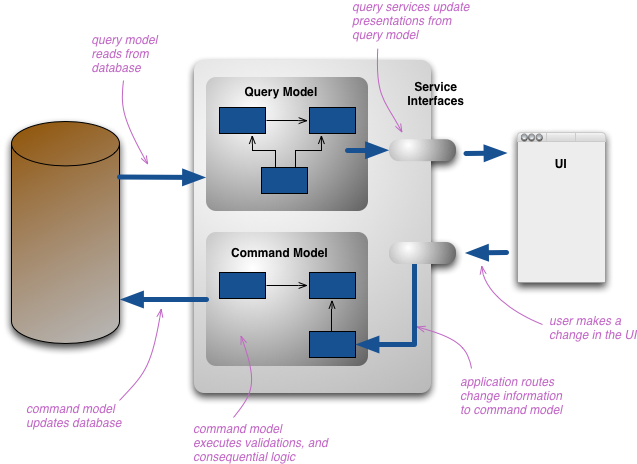
\includegraphics[scale=0.6]{images/cqrs_fowler.png}
    \caption[Schematischer Aufbau eines auf CQRS basierenden Systems]{Schematischer Aufbau eines auf CQRS basierenden Systems.\\Quelle: \cite{fowler_cqrs_2011}}
    \label{fig:cqrs-fowler}
\end{figure}

\section{Vergleich Schichtenarchitektur und CQRS}
\label{sec:vergleich-schichten-cqrs}
Mit Blick auf die Abschnitte~\ref{sec:standard-schichtenarchitektur} sowie \ref{sec:cqrs-pattern}, die einen Einblick in die von Symfony vorgeschlagene Architektur und das CQRS Pattern geben, werden nachfolgend auf die Vor- beziehungsweise Nachteile der beiden Herangehensweisen eingegangen.

\subsection{Vorteile von CQRS}
\label{sub-sec:cqrs-vorteile}
Die Vorteile von CQRS - im Vergleich zu einer gängigen Schichtenarchitektur beziehungsweise der Herangehensweise von Symfony - bauen im ersten Schritt darauf auf, dass komplexe und umfassende Domänen (und die dazugehörigen Prozesse) durch die Verwendung des Patterns gut aufgeteilt werden können. Das Verwenden von \textit{Commands} und \textit{Queries} ermöglicht eine einfache Handhabung der Code-Basis, indem die Wartbarkeit und Erweiterbarkeit verbessert wird. Darüber hinaus kann die Performanz des gesamten Systems durch die Aufteilung der Aktionen in lesende und schreibende Zugriffe verbessert werden und bietet die Möglichkeit, spezifische Anpassungen je Modell vorzunehmen. \parencite[][Seite 240]{ingeno_software_2018}

Die Aufteilung in unabhängige Commands und Queries bietet zudem den Vorteil, dass Applikationen mit einem hohen Performanzanspruch besser eingeteilt und skaliert werden können. Anhand des jeweiligen Anwendungsfalls kann die Last von lesenden und schreibenden Zugriffen unabhängig voneinander getrennt und, sofern notwendig, auch auf mehrere Datenbanksysteme verteilt werden. \parencite[][]{fowler_cqrs_2011}

Sicherheit, beziehungsweise der besser passende, englische Begriff \textit{Security}, ist ein wichtiger Bestandteil moderner (Web-)Anwendungen. Durch CQRS ist es möglich, den Zugriff und das Bearbeiten von Daten genauer einzugrenzen und nur berechtigten Klassen schreibende Aktionen zu erlauben. Dieser Umstand lässt sich im weiteren Verlauf zudem einfacher testen, was bedeutet, dass ungewollte Sicherheitslücken beziehungsweise das Preisgeben von Daten minimiert werden kann. \parencite[][Seite 240]{ingeno_software_2018}

\subsection{Nachteile von CQRS}
\label{sub-sec:nachteile-cqrs}
Neben den Vorteilen, die CQRS mit sich bringt, gibt es jedoch auch Nachteile gegenüber einem Aufbau, der ohne spezifische Auftrennung der Aktionen auskommt (siehe dazu Abschnitt~\ref{sub-sec:standard-funktionsweise} auf Seite \pageref{sub-sec:standard-funktionsweise}).

Für Anwendungen oder APIs, die lediglich einfache \textit{Create}, \textit{Read}, \textit{Update} und \textit{Delete} Funktionalitäten benötigen, stellt die Implementierung von CQRS einen Mehraufwand dar, der womöglich nicht gerechtfertigt ist. Das Pattern bringt zwar die in Abschnitt~\ref{sub-sec:cqrs-vorteile} genannten Vorteile mit sich, die Komplexität des Systems steigt dadurch aber gleichzeitig an und eignet sich daher nicht für alle Anwendungsfälle, oder zumindest nicht für eine Implementierung im gesamten System. \parencite[][Seite 241]{ingeno_software_2018}

Der Vorteil der Auftrennung in Commands und Queries und damit einhergehenden getrennten Datenbanken führt zu einer weiteren Herausforderung, da sichergestellt werden muss, dass diese untereinander konsistent gehalten werden, um nicht unbeabsichtigt mit veralteten Daten zu arbeiten. \parencite[][Seite 241]{ingeno_software_2018}

Heimeshoff und Jander beschreiben weiters den Umstand, dass der Planungs- und Konzeptionsaufwand durch den Einsatz von CQRS bei kleineren Anwendungen nicht direkt im Verhältnis zur Implementierung steht. Die Verlagerung des Fokus muss jedoch nicht unbedingt als ein direkter Nachteil gesehen werden, darf laut ihnen dabei aber nicht außer Acht gelassen werden. \parencite[][]{heimeshoff_cqrs_2013}

Auch Fowler rät von einem unbedachten Einsatz des Patterns ab und betont, dass viele Nutzungsfälle auch mit einem typischen Ansatz ohne Trennung auskommen. \parencite[][]{fowler_cqrs_2011}

\chapter{Umsetzung}
\label{chap:Umsetzung}
Dieses Kapitel beleuchtet nachfolgend die Umsetzung der in Abschnitt~\ref{sec:zielsetzung} auf Seite \pageref{sec:zielsetzung} beschriebenen Ziele anhand von zwei Beispielen und geht dabei genauer auf die technische Herangehensweise sowie Implementierung des CQRS Patterns ein. Anhand der Beispiele wird des Weiteren auf damit verbundene Schwierigkeiten sowie projektspezifische Eigenheiten eingegangen.

\section{Entwicklungsumgebung}
\label{sec:entwicklungsumgebung}
Für die Dauer des Berufspraktikums wurde hauptsächlich die IDE beziehungsweise Entwicklungsumgebung PhpStorm\footnote{\href{https://www.jetbrains.com/phpstorm}{PhpStorm (https://www.jetbrains.com/phpstorm)}} zur aktiven Umsetzung neuer Funktionalitäten im Better Life System verwendet. Selten kam Visual Studio Code\footnote{\href{https://code.visualstudio.com}{Visual Studio Code (https://code.visualstudio.com)}} zum Einsatz, welches aufgrund von persönlichen Präferenzen für das Auflösen von Merge Konflikten, die während des Rebasings aufgetreten sind, eingesetzt wurde.

\smallskip

Aufgrund der Komplexität des gesamten Projektes und der Notwendigkeit eines Servers, welches das PHP Backend zur Verfügung stellt, sind die einzelnen Komponenten (dazu gehören unter anderem ein Webserver, MySQL Datenbanken, ein Cache-Server sowie ein lokaler Mailserver) jeweils in einem Docker Container untergebracht. Mithilfe eines während des Berufspraktikums erstellten \textit{Makefiles}, welches die am häufigsten verwendeten Befehle (unter anderem starten, stoppen und ausführen weiterer Aktionen) beinhaltet, kann die gesamte Applikation samt dem dazugehörigen Frontend lokal aufgesetzt und zur Entwicklung verwendet werden.

Damit zu jedem Zeitpunkt der Entwicklung und auch rückwirkend der jeweilige Stand entsprechend verwendet werden kann, ist ein kompatibler Datenbank Dump in der Git Versionshistorie inkludiert.

\section{Git Branching-Strategie}
\label{sec:git-branching-strategie}
Das Projekt rund um das Better Life System verfolgt, ähnlich wie andere Projekte der Fusonic GmbH, eine möglichst einheitliche und leicht verständliche Git Branching-Strategie, die das Zusammenarbeiten im Team erleichtern soll.

\medskip

Neben einem \textit{stage} und \textit{production} Branch, auf denen die Produktivsysteme mit Kundenzugriff basieren, gibt es einen \textit{master} Branch, der als Ausgangspunkt für alle neu entstehenden Funktionalitäten und Codeänderungen dient. Wenn eine neue Funktion entwickelt oder ein Bug behoben werden muss, wird ein sogenannter \enquote{Feature Branch} erstellt, der alle entsprechenden Änderungen beinhaltet. Nach abgeschlossener Entwicklung wird eine Pull- (oder auch Merge-) Request erstellt, ein entsprechendes Code Review vorgenommen und der Feature Branch schlussendlich in den master Branch gemerged.

\medskip

Die hier beschriebene und beim Better Life System verwendete Herangehensweise orientiert sich am sogenannten \enquote{Git Feature Branch Workflow}. Die Entwicklung von neuen Funktionalitäten sowie Codeänderungen werden in einem Feature Branch gekapselt und sind unabhängig vom master Branch, was ein einafches Zusammenarbeiten ermöglicht. Des Weiteren ist dadurch der Vorteil gegeben, dass der master Branch - durch die Verwendung von jeweils separaten Branches und dazugehörigen Pull Requests - zu jedem Zeitpunkt funktionsfähigen Programmcode beinhaltet. Somit kann dieser für eine entsprechende Veröffentlichung oder als Ausgagspunkt für weitere Branches herangezogen werden. \parencite[]{atlassian_git_2020}

\clearpage

\section{Implementierung von CQRS anhand des \enquote{Region} API Endpunktes}
\label{sec:cqrs-implementierung-region}
Das Better Life System unterscheidet in der Verwaltung von Produkten, der Angebotserstellung und anderweitigen Bereichen im System zwischen verschiedenen Regionen. Um dem Frontend entsprechende Informationen bereitstellen zu können, bedarf es eines API Endpunktes, der diese Informationen zur Verfügung stellt und Änderungen entgegennimmt. Wie die meisten anderen API Endpunkte besteht der \enquote{Region} Endpunkt bereits in der ersten Version (nachfolgend \textit{v1} genannt) beziehungsweise auf Basis der gängigen Schichtenarchitektur (siehe dazu Abschnitt~\ref{sec:standard-schichtenarchitektur} auf Seite \pageref{sec:standard-schichtenarchitektur}).

\smallskip

Im Zuge der Umstellung auf das CQRS Pattern dient die Version 2 (nachfolgend \textit{v2} genannt) des Region Endpunktes als Beispiel für einen einfach umzustellenden Endpunkt, der ansonsten kaum Abhängigkeiten mit sich bringt und repräsentativ für andere Endpunkte ist.

\subsection{Aufbau des v1 Endpunktes}
\label{sub-sec:region-aufbau-v1}
Der bisherige Aufbau des Region API Endpunktes baut darauf auf, dass der entsprechende \texttt{Controller} - welcher schematisch auf auf Seite \pageref{code:region-controller-v1} dargestellt ist und die Anfragen des Frontends von Symfony zugespielt bekommt - einen Großteil der Ablauflogik übernimmt. Dazu gehört - je nach Typ der Anfrage (\enquote{GET}, \enquote{POST}, \enquote{PATCH} etc.) - unter anderem:

\begin{itemize}
    \item Definition der URI des API Endpunktes
    \item Authentifizierung des Benutzers
    \item Zusammentragen benötigter Daten mittels Aufruf des \texttt{RegionManagers}
    \item Serialisierung des \texttt{RegionDto} für eine entsprechende Antwort
    \item Erstellung des tatsächlichen \texttt{Response} Objekts
\end{itemize}

\noindent Der Controller beinhaltet zudem Methoden, die bei der Serialisierung aufgerufen werden und festlegen, welche Attribute nach außen hin benötigt und daher mit Daten befüllt werden müssen.

\begin{listing}[ht]
    \inputminted[fontsize=\footnotesize,linenos,breaklines]{php}{code/region_controller_v1.php}
    \caption[Schematischer Aufbau des v1 \enquote{RegionController}]{Schematischer Aufbau des v1 \enquote{RegionController}}
    \label{code:region-controller-v1}
\end{listing}

\smallskip

Der angesprochene \texttt{RegionManager}, welcher vom Controller aufgerufen wird, um die entsprechenden Daten zu aggregieren, beinhaltet eine Vielzahl an Methoden und Funktionalitäten. Diese umfassen sowohl spezifische Anwendungs- beziehungsweise Businesslogik als auch allgemein gehaltene Funktionalitäten, die über die klassische objektorientierte Vererbung sowie über die von PHP eingesetzten \texttt{Traits} zur Verfügung gestellt werden. Der Einsatz des Managers - der in weiterer Folge das von Doctrine verwendete \texttt{Repository} (in diesem Fall dem \texttt{RegionRepository}) aufruft - hat zur Folge, dass lesende und schreibende Zugriffe in derselben Klasse verwendet und mit sonstiger Businesslogik vermischt werden.

\medskip

Die Abbildung~\ref{fig:region-v1-uml} auf Seite \pageref{fig:region-v1-uml} gibt nochmals einen Überblick über den oben beschriebenen Aufbau des v1 Endpunktes anhand eines grundlegenden UML Diagramms.

\begin{figure}[ht]
    \centering
    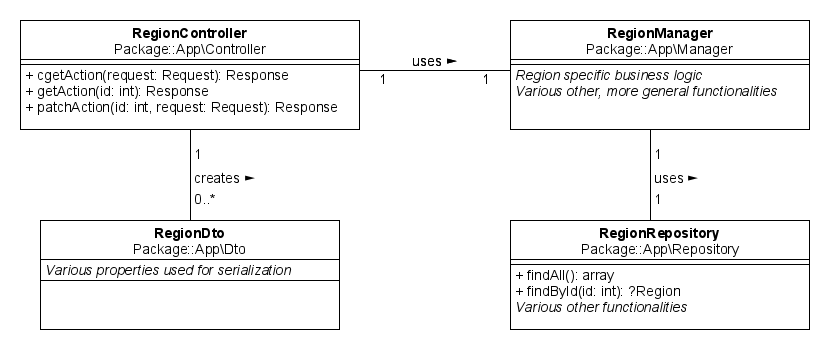
\includegraphics[scale=0.48]{images/region-v1-uml.png}
    \caption[UML Diagramm des v1 \enquote{Region} Endpunktes]{Grundlegender Aufbau des v1 \enquote{Region} Endpunktes samt interner Abhängigkeiten}
    \label{fig:region-v1-uml}
\end{figure}

\subsection{Aufbau des v2 Endpunktes}
\label{sub-sec:region-aufbau-v2}
Für die Umsetzung des CQRS Patterns mit dem Symfony Framework wird im Better Life System auf die von Symfony zur Verfügung gestellte \texttt{Messenger}\footnote{\href{https://symfony.com/doc/4.4/components/messenger.html}{The Messenger Component - (https://symfony.com/doc/4.4/components/messenger.html)}} Komponente zurückgegriffen. Diese ermöglicht es, Commands und Queries in sogenannte \texttt{Envelopes} zu verpacken und von einem entsprechenden \texttt{Command-} beziehungsweise \texttt{QueryHandler} abarbeiten zu lassen. Diese Komponente kommt mit einer Vielzahl von weiteren Funktionalitäten, Konzepten und Patterns, welche im Verlauf dieser Bachelorarbeit jedoch nicht weiter beleuchtet werden.

\clearpage

Die Struktur des in Quellcode~\ref{code:region-controller-v1} auf Seite \pageref{code:region-controller-v1} aufgezeigten Controllers bleibt auch in der CQRS-Version nahezu gleich. Primär verändert sich hierbei die Verantwortung und damit die Größe der einzelnen Methoden, da diese nur noch für die Authentifizierung und Rückgabe der von Symfony benötigten Response zuständig sind. Jegliche weitere Ablauf- und/oder Businesslogik wurde in den jeweiligen Command- beziehungsweise QueryHandler verschoben, um eine strikte Trennung gewährleisten zu können.

\medskip

Der Quellcode~\ref{code:region-v2-structure} auf Seite \pageref{code:region-v2-structure} zeigt den Aufbau der v2 Struktur auf, bei der bereits deutlich die Trennung von Commands und Queries ersichtlich ist, ohne die zugrundeliegende Logik zu kennen.

\begin{listing}[ht]
    \inputminted[fontsize=\footnotesize,linenos]{text}{code/region_v2_structure.txt}
    \caption[Ordnerstruktur des v2 Region Endpunktes]{Ordnerstruktur des v2 Region Endpunktes}
    \label{code:region-v2-structure}
\end{listing}

\subsubsection{Das \enquote{UpdateRegionCommand} und der entsprechende CommandHandler}
\label{sub-sub-sec:update-region-command}
Wie in Abschnitt~\ref{sub-sec:cqrs-grundlagen} auf Seite \pageref{sub-sec:cqrs-funktionsweise} beschrieben, werden schreibende und lesende Aktionen voneinander getrennt. Das Updaten beziehungsweise Aktualisieren einer Region entspricht einer schreibenden Aktion und wird daher mit einem Command abgehandelt.

Ein Command besteht in der im BLS praktizierten Umsetzung aus privaten Attributen und dazugehörigen Gettern und Settern, die öffentlich aufgerufen werden können. Die Daten, die für die Aktualisierung herangezogen werden sollen, sind bereits vom Angular Frontend validiert, werden - wie in Quellcode~\ref{code:update-region-command} auf Seite \pageref{code:update-region-command} ersichtlich ist - jedoch auch noch einmal vom Backend überprüft, um fehlerhafte Eingaben vorzubeugen. Die angewandte Validierung sowie das vorherige setzten der Daten wird hierbei von Symfony in Zusammenspiel mit entsprechenden Erweiterungen vorgenommen.

\begin{listing}[ht]
    \inputminted[fontsize=\footnotesize,linenos,breaklines]{php}{code/update_region_command.php}
    \caption[Die \enquote{UpdateRegionCommand} Klasse]{Die \enquote{UpdateRegionCommand} Klasse}
    \label{code:update-region-command}
\end{listing}

Der zum \texttt{UpdateRegionCommand} dazugehörende CommandHandler umfasst jene Ablauf- und Businesslogik, die sich zuvor im v1 \texttt{RegionController} sowie \texttt{RegionManager} befunden hat und für das Aktualisieren der Daten tatsächlich benötigt wird. Da der Region Endpunkt in der bereits bestehenden Version ohne viel Logik auskommt, spiegelt sich dies auch in der neuen Umsetzung wider, wie der Quellcode~\ref{code:update-region-commandhandler} auf Seite \pageref{code:update-region-commandhandler} aufzeigt.

\pagebreak

\begin{listing}[ht]
    \inputminted[fontsize=\footnotesize,linenos,breaklines]{php}{code/update_region_commandhandler.php}
    \caption[Die \enquote{UpdateRegionCommandHandler} Klasse]{Die \enquote{UpdateRegionCommandHandler} Klasse}
    \label{code:update-region-commandhandler}
\end{listing}

Dem CommandHandler wird, anhand des Typs der beim Formalparameter \texttt{\$command} der \texttt{\_\_invoke} Funktion angeben ist, das entsprechende UpdateRegionCommand von Symfony übergeben. Im weiteren Verlauf wird das bereits bestehende Entity aus der Datenbank entnommen, mit den neuen Daten aktualisiert und entsprechend wieder abgespeichert.

Im Regelfall werden schreibende Aktionen beziehungsweise Commands ohne einen Rückgabewert abgeschlossen. \parencite[]{fowler_commandqueryseparation_2005} In der im Better Life System angewandten Umsetzung wird hierbei jedoch ebenfalls eine Rückgabe in Form einer \texttt{RegionResponse} erzeugt, damit das Frontend die aktualisierten Daten ohne weitere API Aufrufe verwenden kann. Die RegionResponse gleicht Responses anderer v2 Endpunkte und besteht primär aus einer globalen Variable, in der das Entity abgespeichert ist. Zudem beinhaltet sie öffentlich aufrufbaren Getter, die Symfony im Zuge der Serialisierung aufruft, um einen entsprechenden JSON String zu erzeugen.

\subsubsection{Das \enquote{GetRegionQuery} und der entsprechende QueryHandler}
\label{sub-sub-sec:get-region-query}
Das Query, welches genutzt wird um eine Region auszulesen und dem Frontend zur Verfügung stellen zu können, gleicht im Endeffekt dem auf Seite \pageref{code:update-region-command} dargestellten Quellcode~\ref{code:update-region-command}. Bei Queries sind im Regelfall jedoch nur eine globale \texttt{\$id} Variable und gegebenenfalls Werte für die Pagnination (sprich die Unterteilung der Daten auf mehrere, kleinere Blöcke) samt dazugehörigen Gettern und Settern gegeben. Etwaige anderweitige Daten spielen hierbei keine Rolle, da es sich bei einem Query um einen lesenden Zugriff handelt.

\medskip

Ähnlich wie in Abschnitt~\ref{sub-sub-sec:update-region-command} auf Seite \pageref{sub-sub-sec:update-region-command} kommt auch bei einem Query ein entsprechender QueryHandler zum Einsatz, der das Entity aus der Datenbank ausliest und eine \texttt{RegionResponse} als Rückgabewert zur Folge hat. Im direkten Vergleich von Quellcode \ref{code:update-region-commandhandler} (Seite \pageref{code:update-region-commandhandler}) und Quellcode \ref{code:get-region-queryhandler} (Seite \pageref{code:get-region-queryhandler}) ist ersichtlich, dass der \texttt{GetRegionQueryHandler} keinerlei Änderung an bestehenden Daten vornimmt und - wie bei CQRS beschrieben - ausschließlich für einen lesenden Zugriff zuständig ist.

\begin{listing}[ht]
    \inputminted[fontsize=\footnotesize,linenos,breaklines]{php}{code/get_region_queryhandler.php}
    \caption[Die \enquote{GetRegionQueryHandler} Klasse]{Die \enquote{GetRegionQueryHandler} Klasse}
    \label{code:get-region-queryhandler}
\end{listing}

\section{Testen von CQRS anhand des \enquote{ProjectContact} API Endpunktes}
\label{sec:cqrs-implementierung-project-contact}
Der neue \enquote{ProjectContact} Endpunkt, samt der dazugehörigen (Business-)Logik, ist eine verbesserte sowie erweiterte Umsetzung einer in gewissen Teilen bereits bestehenden Kontaktverwaltung. Diese umfasst Personen beziehungsweise Ansprechpartner, die - wie der Name bereits sagt - zu einem Projekt zugehörig sind. Durch die Anforderung des Kunden, dass der Client online sowie offline verwendet werden kann, muss für größere Änderungen an bestehenden API Schnittstellen eine Rückwärtskompatibilität gewährleistet werden.

\medskip

Die tatsächliche Umsetzung aus Sicht von CQRS unterscheidet sich nur wenig von der bereits beschriebenen Herangehensweise und den Charakteristiken, die CQRS im Better Life System aufweist (siehe dazu Abschnitt~\ref{sec:cqrs-implementierung-region} auf Seite \pageref{sec:cqrs-implementierung-region}). Die Schwierigkeit stellt in diesem Fall primär die bestehende Logik im \texttt{ProjectManager}, \texttt{ProjectDto} und anderweitigen Klassen dar, die weiterhin - trotz der intern veränderten Strukturen - entsprechend funktionieren muss.

\medskip

Während dem Arbeiten an den neuen Funktionalitäten und der Einarbeitung der Änderungen in die bestehenden API Schnittstellen spielten die bereits bestehenden Unit Tests - von denen es zum Zeitpunkt des Schreibens dieser Arbeit mehr als 1000 im Better Life System gibt - eine wichtige Rolle bei der Aufrechterhaltung der Rückwärtskompatibilität.

\subsection{Bestehende Unit Tests und ihr Aufbau}
\label{sub-sec:v1-unit-tests}
Die zu einem früheren Zeitpunkt erstellten Unit Tests, die die Logik des \enquote{Project} API Endpunktes (sowie der weiteren Endpunkte) überprüfen, verfolgen alle ein ähnliches Konzept. Zuerst wird eine Anfrage an das PHP Backend simuliert, dann die Antwort beziehungsweise \texttt{HTTP Response} ausgewertet und abschließend auf spezifische Merkmale getestet.

Der Quellcode~\ref{code:project-controller-test} auf Seite \pageref{code:project-controller-test} repräsentiert einen (stark vereinfachten, aber typischen) Test, der vom Aufruf hin bis zur tatsächlichen Antwort und der Anzahl an Datenbankaufrufe alle Komponenten testet und dadurch auf Fehler hindeuten kann.

\begin{listing}[ht]
    \inputminted[fontsize=\footnotesize,linenos,breaklines]{php}{code/project_controller_test.php}
    \caption[Vereinfacht dargestellter v1 Unit Test]{Vereinfacht dargestellter v1 Unit Test}
    \label{code:project-controller-test}
\end{listing}

\subsection{Unit Tests für CQRS Komponenten}
\label{sub-sec:v2-unit-tests}
Im Vergleich zu den \enquote{herkömmlichen} beziehungsweise bisher im BLS eingesetzten Unit Tests testen die auf CQRS ausgelegten Unit Tests deutlich weniger, als - wie bisher - den kompletten Ablauf von simulierter Anfrage bis hin zur Rückgabe. Primär wird auf das Testen der Logik des entsprechenden \texttt{CommandHandler} oder \texttt{QueryHandler} gesetzt, wie der Quellcode~\ref{code:project-contact-queryhandler-test} auf Seite \pageref{code:project-contact-queryhandler-test} aufzeigt.

\medskip

Der Einsatz von deutlich spezifischeren Tests bringt den Vorteil mit sich, dass fehlgeschlagene Tests deutlich präziser darauf hinweisen können, wo Fehler aufgetreten sind. Zudem lässt sich mittels \textit{Mocking} der Einsatz einer tatsächlich existierenden Testdatenbank vermeiden, was die Ausführbarkeit und Performanz deutlich erhöht und externe Fehlerquellen ausschließt.

\begin{listing}[ht]
    \inputminted[fontsize=\footnotesize,linenos,breaklines]{php}{code/project_contact_queryhandler_test.php}
    \caption[Auf das Testen von CQRS ausgelegter Unit Test]{Auf das Testen von CQRS ausgelegter Unit Test}
    \label{code:project-contact-queryhandler-test}
\end{listing}

\clearpage

% Literaturverzeichnis:
\clearpage
\phantomsection
\addcontentsline{toc}{chapter}{Literaturverzeichnis}
\printbibliography

\chapter*{[evtl. Anhang]} % evtl. ersetzen mit \chapter*{Anhang}
\addcontentsline{toc}{chapter}{[evtl. Anhang]} % evtl. ersetzen mit \addcontentsline{toc}{chapter}{Anhang}
Formatvorlage für den Fließtext.

\chapter*{Eidesstattliche Erklärung}
\addcontentsline{toc}{chapter}{Eidesstattliche Erklärung}
Ich erkläre hiermit an Eides statt, dass ich die vorliegende Bachelorarbeit I selbstständig und ohne Benutzung anderer als der angegebenen Hilfsmittel angefertigt habe. Die aus fremden Quellen direkt oder indirekt übernommenen Stellen sind als solche kenntlich gemacht. Die Arbeit wurde bisher weder in gleicher noch in ähnlicher Form einer anderen Prüfungsbehörde vorgelegt und auch noch nicht veröffentlicht.

\vspace{3cm}
\noindent
Dornbirn, am [Datum]\hfill Dominic Luidold

\end{document}
